\section{Towards Generic Parallel Programming}\label{chap:background}

A programming model exposes constrained semantics to the programmer which that programmer uses to express intent. Absent an embedded programming model, the semantics of C-like languages can lead to sequential thinking and execution. Parallel programming models expose parallel semantics to enable developers to create performance portable code. This is commonly achieved by adding semantic value to the base programming language, often referred to as programming with \emph{pragma} annotations. Other methods expose such semantics through library calls or new languages. All three approaches are conceptually suitable to represent programming paradigms such as tasking, parallel patterns and others. Some representatives are the OpenMP programming model~\cite{CITEOPENMP}, threading libraries, or languages like Erlang in which parallelism is a first-class citizen. In general, it is up to the parallel programming model to expose language constructs or library interfaces (APIs) such that they balance convenience to the programmer with semantics sufficient to map the program execution to the parallel computer hardware efficiently and correctly. Questions of what semantic information is needed, what paradigms to present and by what syntactical means span a design space worth taking a closer look at. Figure~\ref{figSemCapture} shows the three areas that constitute a parallel programming model and its design. We call it the semantic capture.

\begin{figure}
\centerline{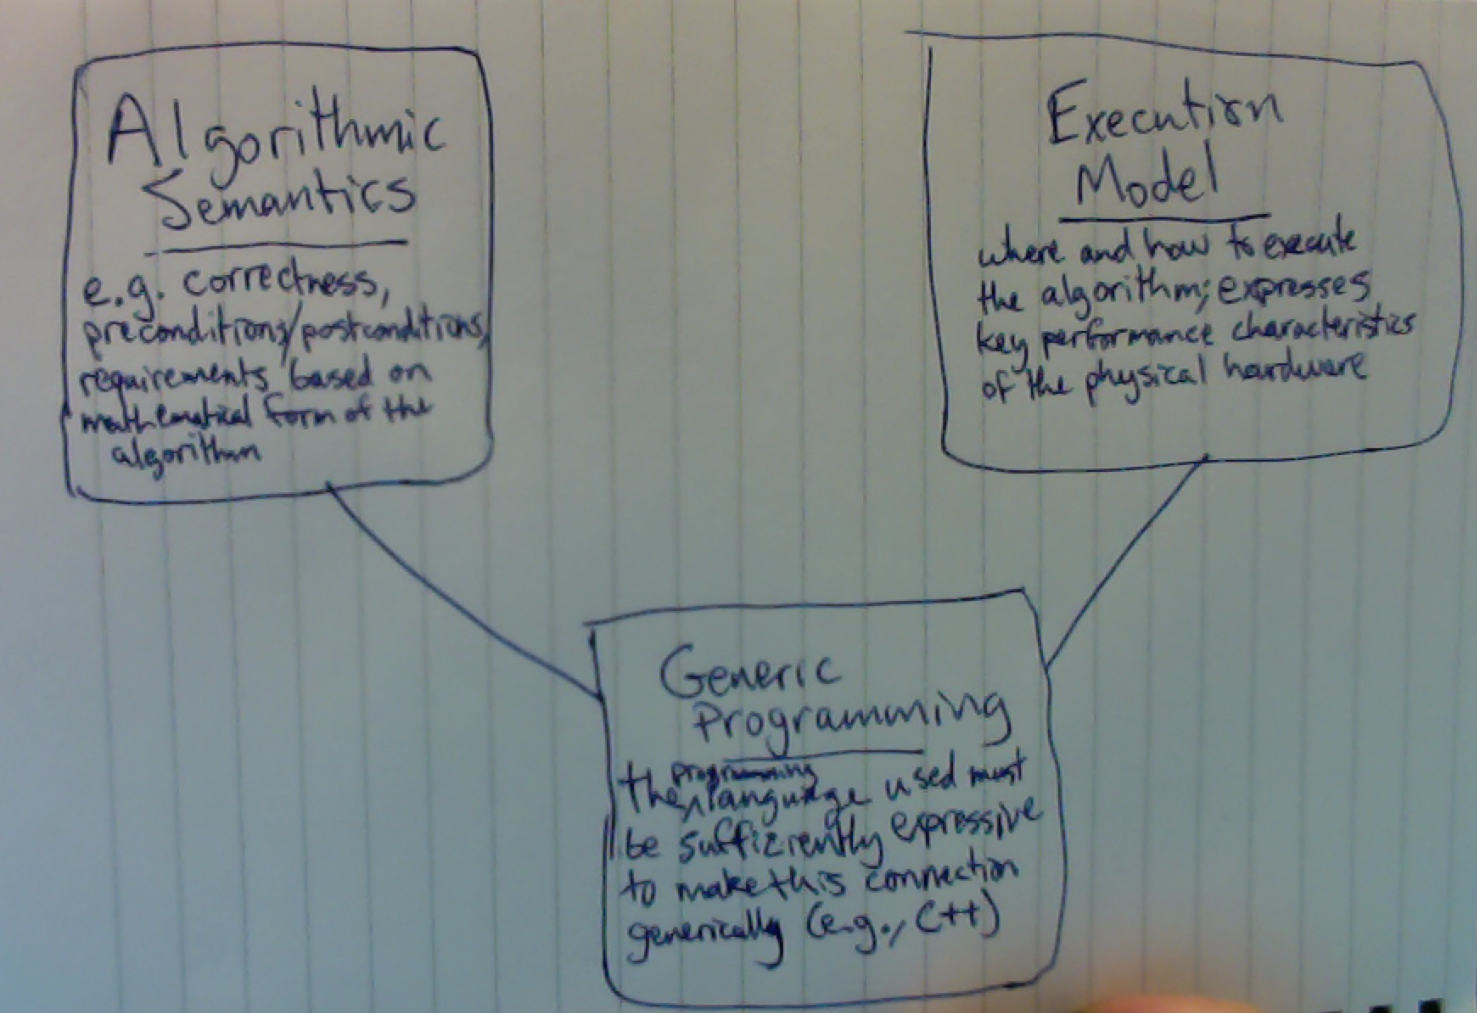
\includegraphics[width=0.45\textwidth]{img/Hollman.png}}
\caption{The Hollman pic :) - placeholder}
\label{fig}
\end{figure}

\begin{figure}[h]
\begin{Verbatim}[frame=leftline]
Semantic information
Paradigm 
Language
\end{Verbatim}
\caption{Semantic capture - a triplet of language, paradigm and semantic information defined by a parallel programming model allow the programmer to express concurrency and the compiler and runtime system to understand and run applications on a parallel machine.}
\label{figSemCapture}
\end{figure}

Semantic information provided by the programmer to the parallel programming model can be grouped into information to express intent and properties. They address the question of \emph{what}, \emph{where} and \emph{how}. In the context of parallel programming, these correspond to defining which code portion to parallelize, where to run and access and how to run that parallel code. Synchronization primitives may be considered as part of the what and information on the execution properties such as data placement or memory access type as the how. Semantics are expressed following a paradigm and a programming language.

The parallel programming paradigm is an abstract ~\emph{representation} with the purpose of facilitating the programmer's understanding of programming rules and program behavior. Which programming paradigm to chose depends on several considerations. Parallel-patterns allow to express concurrency for commonly occurring programming patterns such as loop constructs. Tasking is a paradigm that support the expression of concurrent loops as well as irregular algorithms. Distributed and correctness-oriented programming models may implement actor-based programming. In this programming model, each unit of execution represent an actor who communicates over predefined communication interfaces. This paradigm eliminates accesses to shared state and align well with message passing programming (MPI). The execution model and memory model of a programming model defines behavior. That is, it defines the relationship between abstract concepts and program behavior on the given architecture.

Lastly, a model must decide between declarative and imperative semantics. Declarative semantics require a developer to express intent, implementation is the responsibility of the programming model and underlying toolchain. Imperative semantics require the developer to specify the mechanisms by which their intent will be implemented. In an imperative model, developer success is tied to their knowledge of implementation mechanisms. In a declarative model that success is tied to the developer\'s ability to accurately declare their requirements, and the toolchain\'s ability to turn that into an implementation. Figures~\ref{figOMPLike} and~\ref{figKokkosLike} show examples of two sample applications using the aforementioned types of semantics. While both programming models implement the same programming paradigm (parallel patterns), Figure~\ref{figOMPLike} required the developer to express how to parallelize the loop, while in~\ref{figKokkosLike} the developer just declared their parallel semantics, and relied on the programming model to pick an implementation. 

Kokkos takes the declarative approach. For the developers of our large scientific applications, this is appealing because it allows them to express their algorithms in one way, and rely on Kokkos to map that intent effectively to a variety of architectures. For students this is appealing because they\'re unlikely to have expertise in these architectures. For an educator looking for an implementation vehicle with which to teach students about parallelism, the declarative model eliminates the burden of reimplementing exercises as computer labs and dominant architectures change. For a declarative model to make sense, the educator should know something about the abstract execution model being used to ensure performance portability. Depending on the nature of the course, this could be mostly hidden from students, or discussed in detail.

\begin{figure}
\begin{Verbatim}[frame=leftline]
# pragma model parallel for simd vectorize tile unroll fuse
for ( size_t i = 0; i < N; ++i) {
 /* loop body */
}
\end{Verbatim}
\caption{Declarative parallel programming provides uses pragma annotations to capture semantic information.}
\label{figOMPLike}
\end{figure}

\begin{figure}
\begin{Verbatim}[frame=leftline]
model::parallel_for (N, [=] ( const size_t i) {
  /* loop body */
});
\end{Verbatim}
\caption{Imperative parallel programming uses a base language and relies on programming interfaces to capture information and a documentation that describe their semantics.}
\label{figKokkosLike}
\end{figure}
